%                                             -*- coding: utf-8 -*-
% Mindenkinek csak javasolni tudjuk, hogy latex-et használjon.
% Szakdolgozatnál vagy diplománál már egyértelműen kijönnek az
% előnyei a Worddel szemben.  Ennek ellenére ez a sablon messze nem
% tökéletes.  Ha valamit javítanál benne, kérlek, küld vissza, hogy
% hallgatótársaid is profitáljanak belőle.  Köszönöm.

% További nehézséget okoz, hogy a népszerű latex disztribúciók nem
% tartalmazzák a legújabb változatát a magyar.ldf-nek.  A szükséges
% fájlokat a sablon mellé bemásoltuk, de le is tölthetőek innen:
% http://www.math.bme.hu/latex/
%
%
%
\documentclass[a4paper,oneside]{article}
\usepackage[margin=3cm]{geometry}
% =================================================================
% Magyar nyelvi támogatás
%------------------------
% ###################
% Nyelvváltó parancsok:
%\selectlanguage{english}
%\selectlanguage{magyar}
% rövid angol beszúrás:  \foreignlanguage{english}{some english text}
% határozott névelők generálása ``magyar'' babel-el:
% argumentum+megfelelő határozott nevelő: \az{},\Az{}
% csak a megfelelő határozott nevelő: \az*{}, \Az*{}
% címkék: \aref{}, \aref*{}, képletekhez \aref()
%        \Aref{}, \Aref*{}, képletekhez \Aref()
% oldalak: \apageref{}, \apageref*{}
%        \Apageref{}, \Apageref*{}
% idézetek: \acite, \acite*, \Acite, \Acite*
% ###################
%\usepackage[english,magyar]{babel} %vegyes nyelvi támogatás a
% magyar helyesírás ellenőrzéshez (ispell) és elválasztáshoz
%\selectlanguage{english}

%=================================================================
% direkt ékezetes karakter beírás támogatás
%-------------------------------------------
\usepackage[T1]{fontenc}
\usepackage[utf8]{inputenc}
\usepackage{multirow} 
%================================================================
% Undorító dolog bitmappelt (Type III) betűtípust nézni a PDF-ben
% képernyőn. Az alapértelmezett Computer Modern font LaTex-ben
% bitmappelt, ezért használjunk Times fontot:
\usepackage{times}

%================================================================
% ha ábrát akarunk beemelni, akkor használjuk a graphicx/graphics
% csomagot és az \includegraphics[width=<width>]{abra.pdf} parancsot
\usepackage{graphicx} %for graphics
%kepek helye a gyokerhez(ehhez a file-hoz kepest) kepest
\graphicspath{{./figs/}}
\usepackage{listings}
%================================================================
% Kötelezően használjuk a hyperref csomagot, mert ezzel többek között 
%  kultúrált hyperlinkelt PDF-et lehet csinálni az alábbi
%  variációkban, különféle hyperref backend-ekkel:
%  pdflatex,dvipdfm,ps2pdf
% tapsztalataim szerint a MikTeX (Win32) a 'dvipdfm' konverzióval
% optimális  míg a teTeX (Linux/Solaris) jobb szereti a 'dvips' módszert
%------------------------------------
% pontosan egyet kommentezzünk be!!!!!!!
% értelemszerűen backend függően generáljunk dvi-ból PDF-et!!!
%------------------------------------
% A hyperref csomag az utolsó beolvasott csomag legyen, kivéve néhány
% problémás csomagot, pl. algorithm
%-----------
% ########################### FONTOS ###########################
% A hyperref hibásan működik a babel csomag 'magyar.ldf' fájljának
% 1.5-ös verziójánál korábbi változatával. 2004. februárjában a MikTeX
% és teTex disztribúciók még csak a v.1.4 verziót tartalmazták! A fájl
% aktuális verziója a BME Matematikai intézet LaTeX honlapjáról
% elérhető: http://www.math.bme.hu/latex/ 
% A lusták kedvéért a jelen sablon mellé is mellékelem:
% magyarlatex_0.01-2.tar.gz 
% ########################### FONTOS ###########################
%-----------
\usepackage[colorlinks=true]{hyperref}

%%%%%%%%%%%%%%%%%%%%%%%%%%%%%%%%%%%%%%%%%%%%%%%%%%%%%%%%%%%%%%%%%%%
% Itt kezdődik maga a dokumentum
%%%%%%%%%%%%%%%%%%%%%%%%%%%%%%%%%%%%%%%%%%%%%%%%%%%%%%%%%%%%%%%%%%
\begin{document}
%%%%%%%%%%%%%%%%%%%%%%%%%%%%%%%%%%%%%%%%%%%%%%%%%%%%%%%%%%%%%%%%%%%
% Ezt ne piszkáld!!!!
%%%%%%%%%%%%%%%%%%%%%%%%%%%%%%%%%%%%%%%%%%%%%%%%%%%%%%%%%%%%%%%%%%%
\pagestyle{myheadings} % legyen fejléc 

\newcommand{\onlabcim}{
  \begin{center}
    \huge{\textbf{Project Laboratory Report}}

    \small{Department of Telecommunications and Media Informatics}
  \end{center}
}

% Argumentumok: #1=Név, #2=Neptunkód, #3=szakirány, #4=email, #5 konzulens-1, #6 konzulens-1-email, #7 konzulens-2, #8 konzulens-2-email
\newcommand{\onlabszerzo}[8]{

  \begin{center}
    \begin{tabular}{ r l }
      Author:      & \textbf{#1}                   \\
                   & \href{mailto:#4}{\textbf{#4}} \\
      Neptun-code: & \textbf{\texttt{#2}}          \\
      Department:  & \textbf{#3}                   \\
      Supervisor:  & \textbf{#5}                   \\
                   & \href{mailto:#6}{\textbf{#6}} \\
    \end{tabular}
  \end{center}

}

% % Argumentumok: #1=Név, #2=email
% \newcommand{\konzulens}[2]{
%   \noindent\textbf{Konzulens:} #1 
%   \newline\emph{Email cím:}\/ \href{mailto:#2}{#2}
%   \newline
% 
% }

% Argumentumok: #1=Tanév (xxxx/xx alakban, #2=félév (pont nélkül)
\newcommand{\tanevfelev}[2]{
  \large\noindent\textbf{School year:} #1. school year
  \newline
}

% Argumentumok: #1=téma címe 
\newcommand{\feladatcim}[1]{
  \large\noindent\textbf{Title of the task: #1}
  \bigskip
}

% Argumentumok: #1=téma részletei 
\newcommand{\feladatmaga}[1]{
  \large\noindent\textbf{Task:}
  \newline
  #1
  \newline
  \smallskip
}

% A fejezetek közé beágyazott irod.jegyzék
\def\thebibliography#1{\renewcommand{%
    \baselinestretch}{1}\subsection{Used references}\list
  {\small [\arabic{enumi}]}{\settowidth\labelwidth{[#1]}\leftmargin\labelwidth
    \advance\leftmargin\labelsep
    \usecounter{enumi}}
  \def\newblock{\small \hskip .11em plus .33em minus .07em}
  \sloppy\clubpenalty4000\widowpenalty4000
  \sfcode`\.=1000\relax}
\let\endthebibliography=\endlist%


%%% Local Variables: 
%%% mode: latex
%%% TeX-master: "template"
%%% End: 
 % Ez kell!!!
\markright{Kiss Dániel Márk (WP871Q)} % egyoldalas fejléc!!!
%--------------------------------------------------------------------
% fedlap
%--------------------------------------------------------------------
\begin{titlepage}
  %bme logo 
  \begin{figure}[h]
    \centering
    
\includegraphics[width=12cm]{bme_logo}
    \label{fig:bme_logo}
  \end{figure}
  \thispagestyle{empty}
  %cím generálás
  \onlabcim

  % \begin{center}
  %   \begin{tabular}{ p{3cm} p{5cm} }
  %   
  %   Készítette: & Beszámoló Péter  \\
  %   Neptun-kód: & BPOX43  \\
  %   Ágazat: & Médiainformatika  \\
  %   E-mail cím: & b.peter@onlab.hu  \\
  %   Konzulens: & Dr. Péhádes István  \\
  %   E-mail cím: & pehades@tmit.bme.hu  \\
  %   Konzulens: & Doktor Andusz  \\
  %   E-mail cím: & doktora@tmit.bme.hu  \\
  %   
  %   \end{tabular}
  % \end{center}


  %\szerzo argumentumok: #1=Név, #2=Neptunkód, #3=szakirány, #4=email,#5 konzulens-1, #6 konzulens-1-email, #7 konzulens-2, #8 konzulens-2-email
  \onlabszerzo{Kiss Dániel Márk}{WP871Q}{Business Informatics}{daniel.mark.kiss@gmail.com}{Dóka János}{doka.janos@tmit.bme.hu}


  %\feladatcim argumentuma a feladat rövid, 1 soros címe
  \feladatcim{Augmented reality application for economic metrics visualization}

  %\feladatmaga argumentuma a feladat 1-2 bekezdésnyi ismertetése
  \feladatmaga{During the 14 weeks of the self-contained laboratory I am going to implement an economic visualization AR based application. With the application users can visualize the requested data using augemented reality technologies. Main purpose of the project is to get to know about the current frameworks and technologies in these growing field.
  }


  %\tanevfelev argumentumok:
  % #1=Tanév (xxxx/xx alakban), #2=félév (pont nélkül!)

  \tanevfelev{2023/24}{I}

\end{titlepage}

%==================================================================
\section{Introduction}
\label{sec:kornyezet}
% A munka  előzményei és kiindulási állapota
% \newpage
\label{sec:bevezeto}


Smartphones have become a defining part of our days. By now we can't even imagine our everyday life without them. We read e-mails, browse the Internet or monitor daily exchange rates. Now we can do all important things with our phones. Listening to music and watching series, but in terms of photography and video capabilities, they are not far behind cameras designed for professional purposes. Their computing capacity has grown exponentially over the years, but that was true only for the firt ten years of the industry. The quality of camera systems is also undergoing significant progress every year.Perhaps this is why many people say that the development of telephones is starting to slow down. This industry has reached its peak.

At the time, in 2007, the iPhone was considered a huge world sensation and now we know it was a world-changing announcement. At the time of writing this report, there are several reports that Apple is working on the introduction of a similarly large and decisive new product line. The so-called Apple AR/VR glasses. Only time will tell if this really happened until then I thought that it would be a great advance if I started familiarising with this technology. If this will be the next "touchscreen phone era", I thought it would be worthwhile to start dealing with it in time. Regardless, I have long been interested in the technology's operating principle and scope of use. From the consumer side, what kind of application possibilities does augmented reality technology have? At that time, I wanted to implement a similar augmented reality-like navigation system in my own high school navigation application. Unfortunately, I did not know about the existence of these technologies at the time.

As I mentioned in the first paragraph, today's phones have a huge computing capacity. This is also why it is possible for such augmented reality applications to run on our phones. Based on the 1 or better case 2 or 3 lenses placed in the phone, it can measure the 3D depth of each scenario. There are phones, such as the iPhone 13 Pro, which have a laser LiDAR sensor placed specifically for this purpose. In the 2010s, many devices with similar technology came out, such as Microsoft's Kinect developed for the X-Box 360 console. It is also worth mentioning Google Glass developed by Google or HoloLens and HoloLens 2 marketed by Microsoft. Unfortunately, the former mentioned Google Glass was not an undivided success and in 2023 the sale of the glasses was discontinued.

Last but not least, it is important to mention the Oculus Quest 2 VR headset introduced by Meta and the computer use and games based on it. In addition, the Metaverse, announced by Meta 2 years ago, is also an important milestone in the life of virtual reality and therefore also in the life of augmented reality.

As the examples above clearly reflect, it will be an important and presumably defining technology in the future. In light of this, during my self-lab, I got to know the ARKit and RealityKit developed and used by Apple. And with the help of the frameworks, I developed an augmented reality application displaying economic metrics. It helped me to reach my goal significantly faster with it. The pre-defined classes and functions lifted the heavy part of the work from my shoulders. And during the report I used LaTex, because I felt it was time to familiarize myself with this kind of documentation language.

\newpage
%==================================================================
\section{Current techologies}
\label{sec:az-elvegzett-munka}

Before I started the development of the application I have done a research period to have a better overview of the current market \cite{microsoftAr}.
There are several frameworks to choose from to start developing augmented reality applications. The most used AR frameworks are Google ARCore, Apple ARKit and RealityKit, Simple CV and Unity AR Foundation \cite{appleAr} \cite{appleArRealityKit}.
I ended up using Apple ARKit to build my app. I've been working with iOS development for several years and I'm sure with the Swift language as well.


\subsection{Unity}
\label{sec:a-munkam-ismert}

One of the main frameworks that we can use if we want to develope augmented reality application is Unity.
Unity is a purpose-build framework for augmented reality development.  It's key feature is that with the framework developer can easily deploy it's product across multiple mobile and wearable AR devices. It includes core features from ARKit(Apple), ARCore(Google) and HoloLens(Microsoft) as well unique features \cite{unity}.

AR Foundation which is the recommended framework for Unity development there are several features what the developers can use like:
\begin{itemize}
  \item Device tracking
  \item Raycast
  \item Plane detection
  \item Gestures
  \item Face tracking
\end{itemize}

\subsection{Apple ARKit and RealityKit}

Apple ARKit \cite{appleArKit} and RealityKit \cite{appleArRealityKit} are two powerful technologies developed by Apple that enable the creation of immersive augmented reality experiences on iOS devices. ARKit is a software framework that provides developers with the tools and resources they need to build augmented reality apps for iPhones and iPads. It allows developers to easily place virtual objects in the real world, track the user's position and orientation, and integrate real-time camera data to create realistic and interactive experiences.

On the other hand, RealityKit is a high-level framework that makes it easy for developers to create 3D content and build AR experiences without requiring extensive knowledge of 3D graphics or game engine programming. RealityKit includes features such as physics simulations, animations, and spatial audio, which can be used to create highly immersive AR experiences.

Together, ARKit and RealityKit provide developers with a comprehensive set of tools for building augmented reality experiences on iOS devices. With these technologies, developers can create innovative and engaging apps that allow users to interact with virtual objects in the real world, opening up new possibilities for gaming, education, and more.

ARKit detects the real-world and with the help of RealityKit it projects the virtual object on the scene. As we can see on the example below \ref{fig:arKitRealityKit} the real world table is detected by ARKit and after that it can be used in RealityKit to compose the scene with the added virtual sphere in it.

\begin{figure}[!ht]
  \centering
  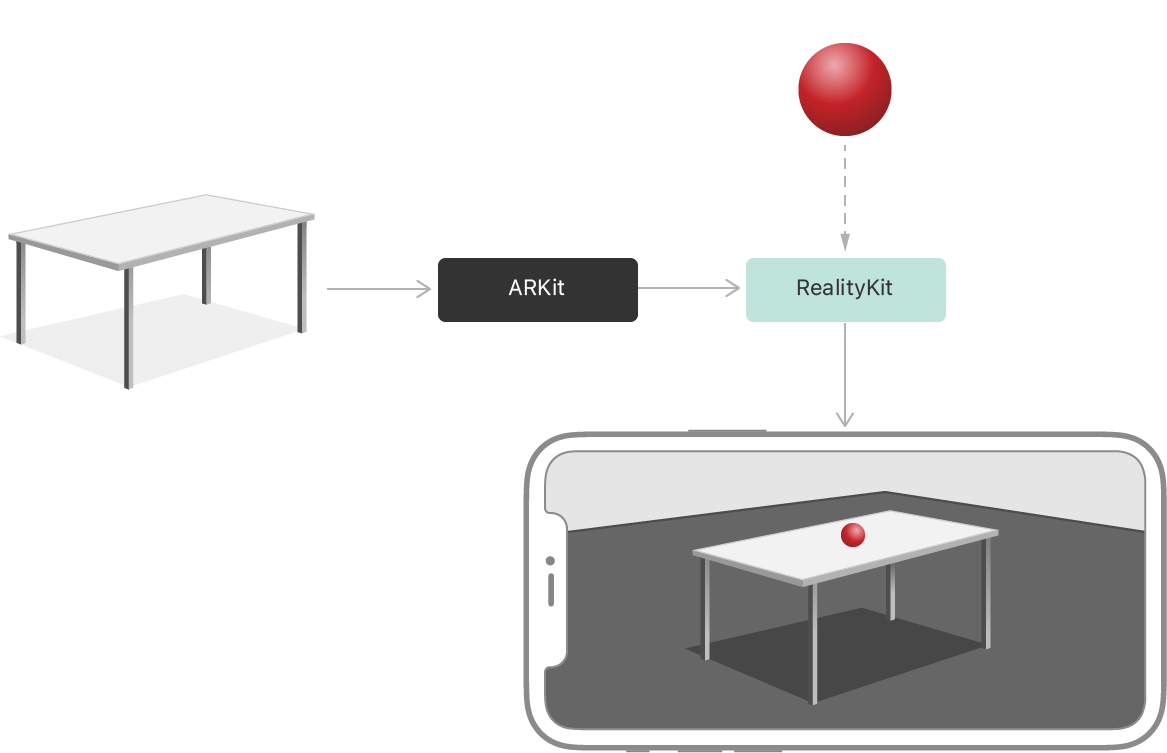
\includegraphics[width=150mm]{../images/realitykit.png}
  % \includegraphics[width=150mm, keepaspectratio]{figures/TeXnicCenter.png}
  \caption{RealityKit and ARKit usage.}
  \label{fig:arKitRealityKit}
\end{figure}

RealityKit’s features:
\begin{itemize}
  \item Rendering: RealityKit offers a powerful new physically-based renderer built on top of Metal, which is fully optimized for all Apple devices.

  \item Animation: It has built-in support for Skeletal animation and Transform-based animation. So, if you want, you can animate anithing or you can move, scale and rotate objects with various easing functions.

  \item Physics: With a powerful physics engine, RealityKit lets you adjust real-world physics properties like mass, drag and restitution, allowing you to fine-tune collisions.

  \item Audio: Spacial audio understanding and automatic listener configuration let you attach sound effects to 3D objects. You can then track those sounds, making them sound realistic based on their position in the real world.

  \item ECS: From a coding perspective, RealityKit enforces the Entity Component System design pattern to build objects within the world.

  \item Synchronization: The framework has built-in support for networking, designed for collaborative experiences. It even offers automatic synchronization of entities between multiple clients.
\end{itemize}


\subsection{SwiftUI}

SwiftUI is Apple's brand new framework for building user interfaces for iOS, tvOS, macOS, and watchOS.
Apple introduced SwiftUI in 2019 and the framework has been evolving ever since.
Unlike UIKit, SwiftUI is a cross-platform framework. The key difference with UIKit and AppKit is that SwiftUI defines the user interface declaratively, not imperatively.
What does that mean?

Using UIKit you create views to build the view hierarchy of your application's user interface. That is not how SwiftUI works. SwiftUI provides developers with an API to declare or describe what the user interface should look like. SwiftUI inspects the declaration or description of the user interface and converts it to your application's user interface. SwiftUI does the heavy lifting for you.

This declarative approach in SwiftUI simplifies the process of building user interfaces by allowing developers to focus on describing the desired outcome rather than manually managing the view hierarchy. Instead of writing code that specifies how each UI element should be positioned and styled, developers can define the structure and appearance of their user interface using SwiftUI's intuitive syntax.

One of the powerful features of SwiftUI is its ability to provide real-time previews of your user interface while you are designing it. As you make changes to the code, the preview updates automatically, allowing you to see the immediate impact of your modifications. This live preview feature accelerates the development process by providing instant feedback and reducing the need for constant recompilation.

SwiftUI also offers seamless integration with other Apple frameworks and technologies. For example, you can easily incorporate augmented reality experiences using ARKit or leverage the power of Core ML for machine learning tasks within your SwiftUI-based app. This level of integration allows developers to leverage the full potential of Apple's ecosystem while building their user interfaces.


\newpage
\section{Development}

The AR app is designed to retrieve real-time economic data from an API and display it to the user in an augmented reality environment. The app provides users with the ability to interact with the data, manipulate its presentation, and perform various actions.

Upon launching the app, the user will have access to a selection of economic indicators and financial data. The app will establish a connection with the designated API to fetch the latest information in real-time.
This data can include stock market indices, currency exchange rates, inflation rates, and other relevant economic metrics.

The user can choose to view the data in chart representation.
The app will offer a range of customization options, allowing the user to rotate, reposition, and manipulate the visual elements to suit their preferences.
The app's potential for expansion and enhancement is virtually limitless. Developers can continuously add new economic data sources, expand the available indicators, introduce advanced analytics and forecasting capabilities, integrate social media sentiment analysis, and incorporate machine learning algorithms to offer personalized insights and recommendations to users.
\subsection{Development process}
For the development phase of the project I used Apple's XCode integrated developer environment(IDE) as the main developer platform for iOS and ARKit development. For testing I used an iPhone 11 with dual camera system.
I have also version controled the whole development process using git and publishing it on GitHub. Not only the source code can be found there but also the documentation of this project as I have writen it using \LaTeX{}.

\subsection{APILayer Rest API}

The fundamental part of the application is the data it displays. For retriving the displayed informations I used APILayer's Exchange Rates Data API an open and available for free financial API.  The only problem is that you can only do 250 queries per month in the free version. I used 2 endpoints. The first is '/convert' \ref{listing:convertEndpoint}. With this endpoint, we have any amount conversion from one currency to another. The output of this enpoint is the following JSON.

\begin{lstlisting}[frame=single,float=!ht,caption=JSON from /convert endpoint, label=listing:convertEndpoint]
  {
    "success": true,
    "query": {
        "from": "EUR",
        "to": "HUF",
        "amount": 1
    },
    "info": {
        "timestamp": 1682930463,
        "rate": 373.180303
    },
    "date": "2023-05-01",
    "result": 373.180303
  }
\end{lstlisting}

The other endpoint used is '/fluctuation' \ref{listing:fluctuationEndpoint}. This endpoint returns the fluctuation data between specified dates. The data can be for all available currencies or for a specific set.


\begin{lstlisting}[frame=single,float=!ht,caption=JSON from /fluctuation endpoint, label=listing:fluctuationEndpoint]
{
  "base": "EUR",
  "end_date": "2018-02-26",
  "fluctuation": true,
  "rates": {
    "JPY": {
      "change": 0.0635,
      "change_pct": 0.0483,
      "end_rate": 131.651142,
      "start_rate": 131.587611
    },
    "USD": {
      "change": 0.0038,
      "change_pct": 0.3078,
      "end_rate": 1.232735,
      "start_rate": 1.228952
    }
  },
  "start_date": "2018-02-25",
  "success": true
}
\end{lstlisting}

%\cite{apilayer}
\newpage
\subsection{Visualization}


One of the most challenging aspects of user interface development is synchronizing the application's state and its user interface. Every time the application's state changes, the user interface needs to update to reflect the change. During the development phase, this was a challenge that had to be overcome. Despite the fact that I have already used and developed an iOS application with SwiftUI, it was excellent practice to deepen my knowledge of user state management. I used ObservableObjects to solve this problem.

I used a common state management technique, the MVC pattern, to control the data and model. MVC (Model-View-Controller) is a pattern in software design commonly used to implement user interfaces, data, and controlling logic. It emphasizes a separation between the software's business logic and display. This "separation of concerns" provides for a better division of labor and improved maintenance.  Sticking to convention, I created a CurrencyController, CurrencyView and a CurrencyModell class. The CurrencyModel class contains the generated 3D models and their associated values. The task of the CurrencyController class is to query the data and update the information displayed on the View. In the CurrencyView class, it deals with the code defining the appearance of the application and the display of the given dataset \cite{mozilla}.

To operate augmented reality and display the 3D generated graph, I used the ARKit and RealityKit frameworks provided by Apple.

The CurrencyARViewContainer is responsible for displaying the AR view.

To generate the texts and columns, I used the .generateBox() and .generateText() functions of the built-in MeshResource class.
The MeshResource class stores the points defining the shapes. In order for this to become a 3D model, a texture must also be specified. I used the SimpleMaterial() function for this.
We also need an AnchorEntity, which defines the center of our model in the 3D world.
After defining these variables, we can create the ModelEntity and place it in the AR world using the AnchorEntity.


To be able to move the different elements together, all 3D models are children of the axes. Thus, if the axis moves, the connected elements will also move due to the parent-child relationship. In its current version, MeshResource does not support the generation of cones by default, so I was able to achieve this by using an external library package. After importing the RealityGeometries library, I was able to easily generate cones, which I eventually used to draw axes.
%%%%%%%%%%%%%%%%%%%%%%%%%%%%%%%%%%%%%%%%%%%%%%%%%%%

After the application launches the camera opens and show the real world for the user.  With the bottom selector the user can select which currency he/she  would like to display as Figure \ref{fig:selector} presents.
After he/she decided which currency should be displayed a confirmation button appeares as it is displayed on Figure \ref{fig:megerosites}. If the green tick is touched then the graph shows up with the correct current informations.

The camera function in the application allows you to capture the current state of the graphs, which in this case came in handy for documentation.
\begin{figure}[!ht]
  \centering
  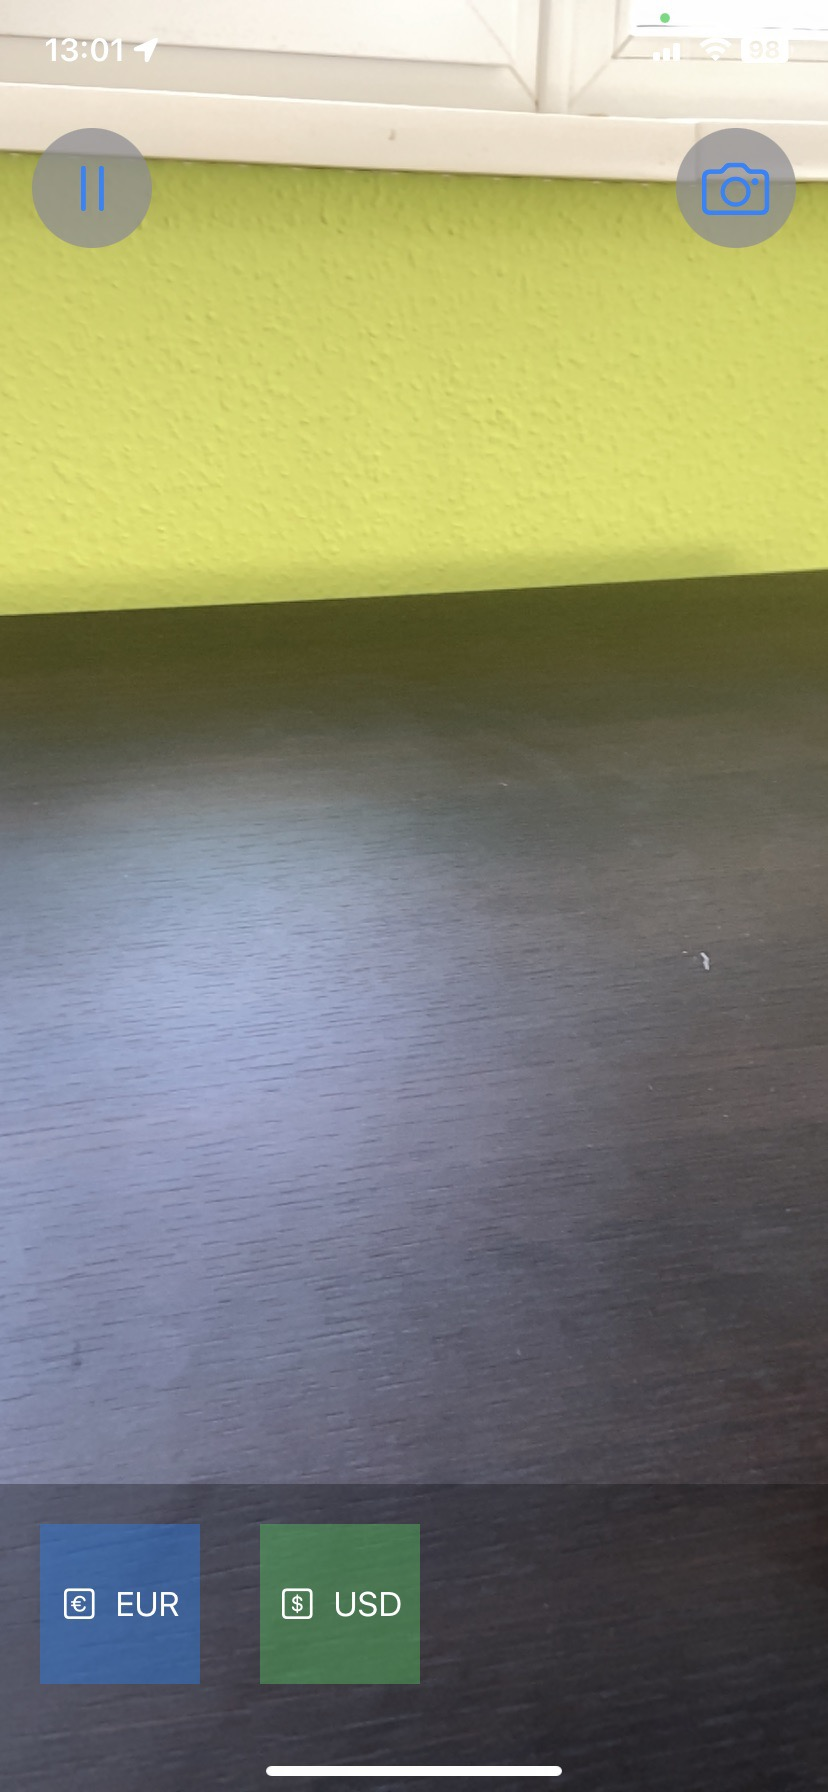
\includegraphics[height=75mm, keepaspectratio]{../images/selector.jpeg}
  % \includegraphics[width=150mm, keepaspectratio]{figures/TeXnicCenter.png}
  \caption{Selector UI part.}
  \label{fig:selector}
\end{figure}

\begin{figure}[!ht]
  \centering
  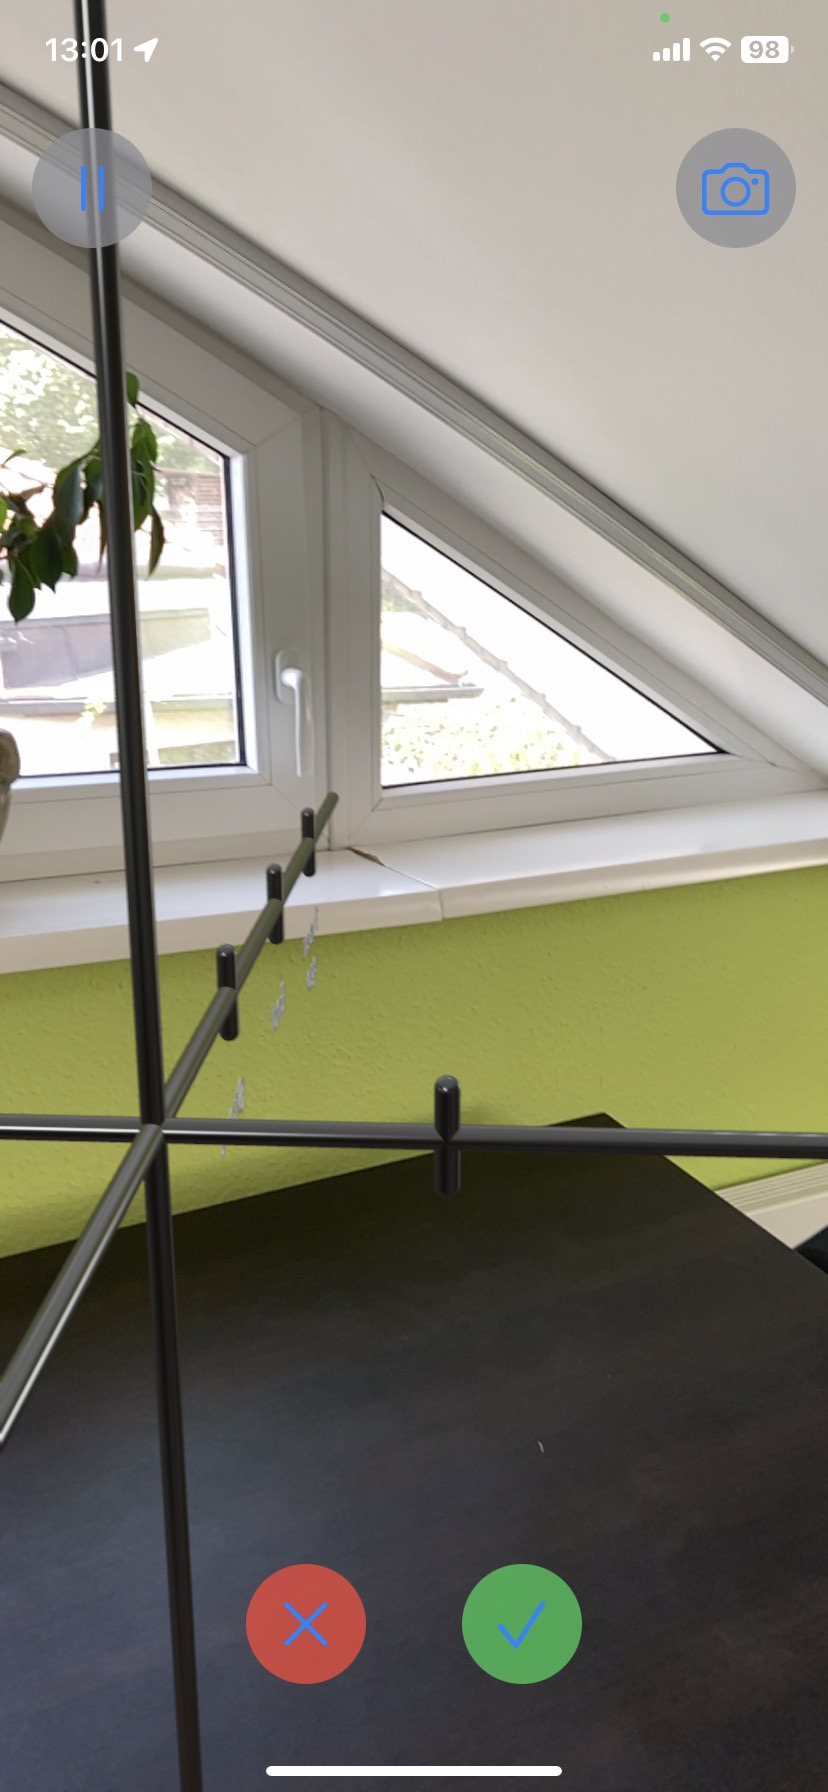
\includegraphics[height=75mm, keepaspectratio]{../images/megerosites.jpeg}
  % \includegraphics[width=150mm, keepaspectratio]{figures/TeXnicCenter.png}
  \caption{Confirmation buttons.}
  \label{fig:megerosites}
\end{figure}


\begin{figure}[!ht]
  \centering
  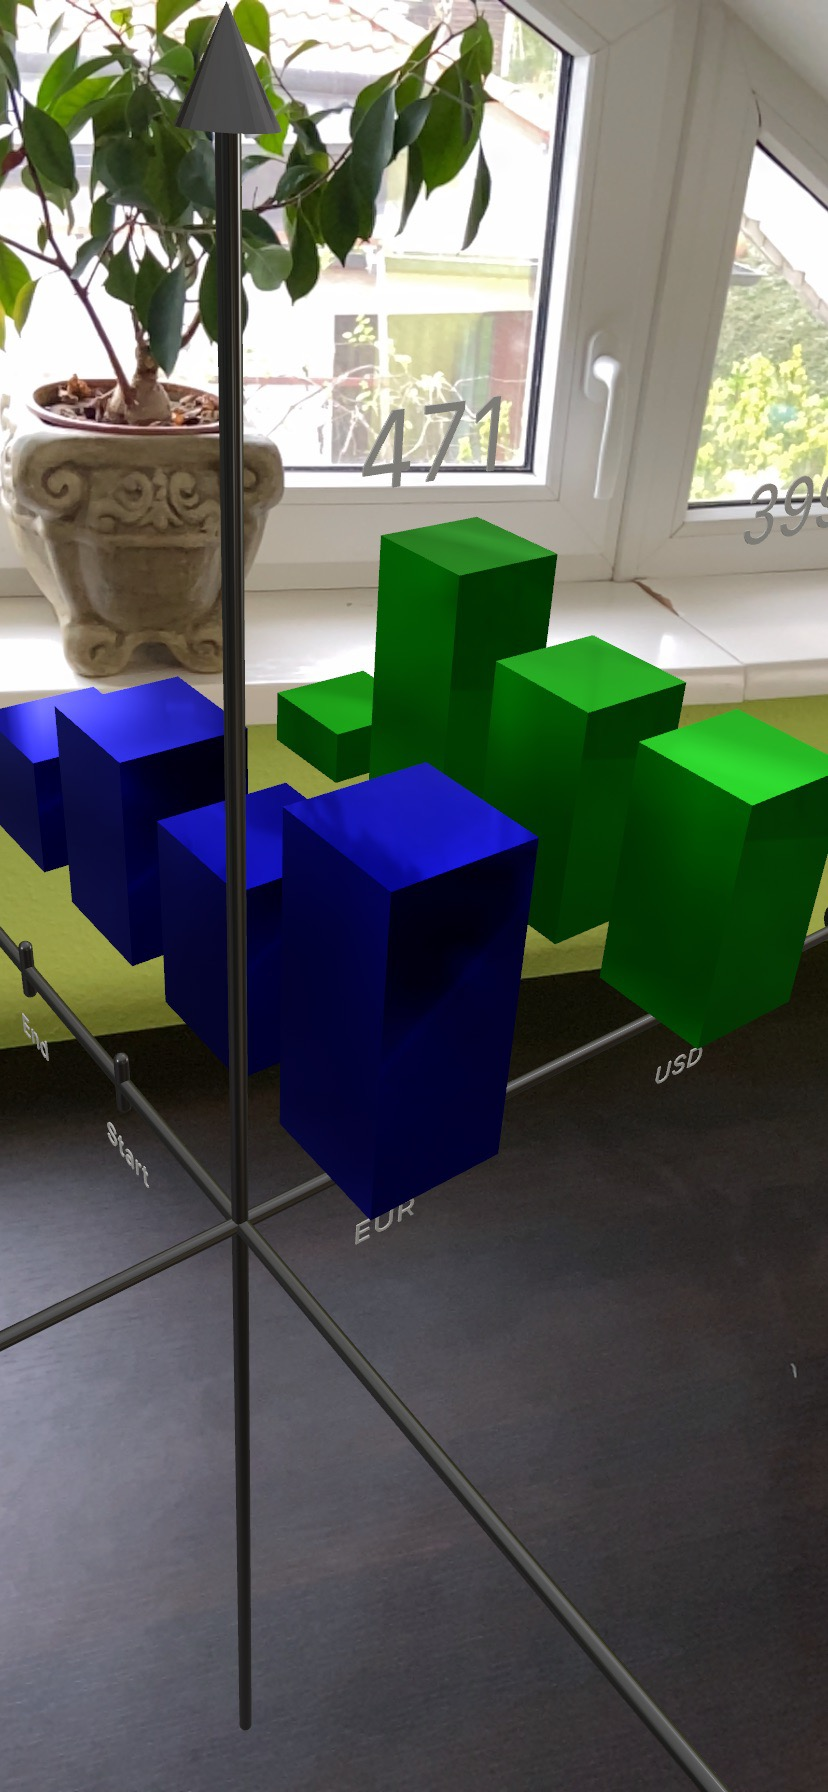
\includegraphics[height=75mm, keepaspectratio]{../images/top.jpeg}
  % \includegraphics[width=150mm, keepaspectratio]{figures/TeXnicCenter.png}
  \caption{The visualized graphs.}
  \label{fig:top}
\end{figure}

As the attached images clearly show, the virtual 3D graph can be easily walked around and viewed from different angles as we see it on Figure \ref{fig:top}., thereby giving users a new comparative perspective. It is possible to move and rotate the entire graph, as well as move the current exchange rate columns to make it easier to compare with other metrics. The move and rotate functions are only available in Spectate mode, for this you have to stop Live mode (or otherwise start Live mode) by pressing the button located in the upper left corner.

Currently, 2 currencies are available in the application, but of course this can be easily expanded at any time in the future. These two are EUR to HUF and USD to HUF. These can be displayed after selection and confirmation from the bottom bar. If the given exchange rate is already placed, it can no longer be added to the graph twice.

For the currencies currently only the EUR and USD are available. Both rates are convert to HUF refered to 1 unit.The blue column represents the EUR while the green columns shows the USD values.

On the Z axes the user can visualize and start and the end fluctuation for the past 10 days. The last column shows the one year ago value of the givne currency.
In addition to the Z-axis functionality, I have also implemented interactive controls for manipulating the graph itself.
By enabling users to move and rotate the entire graph, they have the flexibility to view the data from different angles and perspectives. This interactive capability is achieved by grabbing the X-axis and performing the appropriate finger gesture on the screen, providing a tactile and intuitive method for exploring the data.
Furthermore, the ability to move and rotate the graph allows for a more immersive and customizable experience. Users can adjust the graph's position and orientation to suit their preferences, making the app feel more personalized and tailored to their individual needs.






\section{Summary and future work}
\label{sec:osszefoglalas}

The main focus of my independent lab topic was augmented reality. I was interested in how it works and where the technology currently stands.
The field of augmented reality (AR) has witnessed significant advancements in recent years, and its potential for growth and innovation continues to expand. During my independent lab project, I delved into the intricacies of AR technology and closely examined its current state. In this pursuit, I focused specifically on Apple's ARKit and RealityKit, which are widely recognized as powerful tools for AR development.
Exploring ARKit and RealityKit allowed me to gain comprehensive knowledge of their capabilities and how they can be leveraged in real-world applications. Additionally, my project provided an opportunity to deepen my understanding of SwiftUI, which complements AR development by providing a declarative and intuitive approach to building user interfaces.
\linebreak
It was challenging to start this project because there were only a few good sources to educate myself from. Thankfully when I had any doubt my supervisor helped me.
In the future the app will provide additional features to enhance the user experience.
For example, it can offer historical data analysis, allowing users to compare current economic data with past trends. It can also include tools for creating personalized portfolios, setting up alerts for specific data thresholds, or conducting virtual simulations to predict the potential impact of economic events.
\linebreak
Overall, the AR app serves as a dynamic platform for users to access and interact with real-time economic data in an immersive and customizable manner, with endless possibilities for future growth and innovation.
It was also a good starting point if I ever want to continue my journy I have a begining point. For the time being it is totaly enough for me.
\linebreak
Curretly from my point of view it is a very immature in a sense that the big companies can't even produce any remarkable augmented reality applications for the smartphones. Major companies are yet to unleash the full potential of augmented reality applications, indicating that there is still much to be explored and discovered. All in all I think it has huge potentials in it but it's market is yet to be reveald. Perheaps with the launch of the commercial augemented reality glasses? Who knows. Only time will tell.
\newpage

%==================================================================
\section{Bibliography}
\label{sec:irod-es-csatl}

\begin{thebibliography}{9}
  \label{sec:tanulm-irod-jegyz}

  \bibitem{microsoftAr} Microsoft authors, \emph{What is Augmenteted Reality}, 2023 May 26.  Available
  from: \\ \url{https://dynamics.microsoft.com/en-us/mixed-reality/guides/what-is-augmented-reality-ar/}

  \bibitem{appleAr} Apple authors, \emph{Augmented Reality}, 2023 May 26.  Available
  from: \\ \url{https://developer.apple.com/augmented-reality/}

  \bibitem{appleArRealityKit} Apple authors, \emph{Reality Kit}, 2023 May 26.  Available
  from: \\ \url{https://developer.apple.com/documentation/realitykit/}

  \bibitem{appleArKit} Apple authors, \emph{Augmented Reality}, 2023 May 26.  Available
  from: \\ \url{https://developer.apple.com/documentation/arkit}

  \bibitem{unity} Unity authors, \emph{AR Foundation}, 2023 May 26.  Available
  from: \\ \url{https://unity.com/unity/features/arfoundation}

  \bibitem{mozilla} Mozilla authors, \emph{What is MVC}, 2023 May 26.  Available
  from: \\ \url{https://developer.mozilla.org/en-US/docs/Glossary/MVC}


\end{thebibliography}
%==================================================================
\end{document}
%%% Local Variables: 
%%% mode: latex 
%%% TeX-master: t 
%%% End:

